% =====================================================================
%  MiniFrontier: A 14.6M-Parameter Monolingual Arabic Language Model
%  ---------------------------------------------------------------
%  COMPILE INSTRUCTIONS (do not run locally per author request):
%    Recommended : pdflatex  ->  pdflatex   (two passes, for refs/TOC)
%    Arabic glyphs in the appendix sample render as boxes under
%    pdflatex. If you want the Arabic generation sample to render,
%    compile with XeLaTeX or LuaLaTeX and uncomment the polyglossia
%    block flagged below (search "XELATEX-ARABIC").
%  Dependencies: pgfplots, booktabs, amsmath, hyperref, geometry,
%                xcolor, caption, multirow, array, graphicx.
%  ---------------------------------------------------------------
%  MEASURED, NOT ESTIMATED (updated 2026-06-23):
%    - Bits-per-byte (Sec. "Measured bits-per-byte", label sec:bpb): BPB=1.25,
%      from per-token UTF-8 byte lengths + mask-aware val CE. Source: measure_bpb.py
%      -> bpb_results.json.
%    - Data-ceiling scaling sweep (Sec. label sec:ceiling): scaling_sweep.py ->
%      scaling_results.json + scaling_curve.png (figure auto-included via
%      \IfFileExists once the RTX-3090 run completes; harness validated on 5M pilot).
%    - The 3.5-nat floor is softened to a projection, not a settled target.
% =====================================================================
\documentclass[10pt,twocolumn]{article}

\usepackage[utf8]{inputenc}
\usepackage[T1]{fontenc}
\usepackage{geometry}
\geometry{a4paper, margin=1.9cm, columnsep=0.7cm}
\usepackage{amsmath,amssymb}
\usepackage{booktabs}
\usepackage{array}
\usepackage{multirow}
\usepackage{xcolor}
\usepackage{graphicx}
\usepackage{caption}
\captionsetup{font=small,labelfont=bf}
\usepackage{pgfplots}
\pgfplotsset{compat=1.17}
\usepackage{pgfplotstable}
\usepackage[colorlinks=true,linkcolor=blue!55!black,citecolor=blue!55!black,
            urlcolor=blue!55!black]{hyperref}
\usepackage{authblk}
\usepackage{abstract}

% ---- accent palette ----
\definecolor{mfblue}{RGB}{31,86,140}
\definecolor{mfred}{RGB}{176,42,55}
\definecolor{mfgreen}{RGB}{34,120,80}
\definecolor{mfgray}{RGB}{120,120,120}
\definecolor{mforange}{RGB}{200,110,30}

% ===== XELATEX-ARABIC (optional) =====================================
% To render the Arabic generation sample, compile with XeLaTeX and
% uncomment the four lines below:
% \usepackage{polyglossia}
% \setmainlanguage{english}
% \setotherlanguage{arabic}
% \newfontfamily\arabicfont[Script=Arabic]{Amiri}
% =====================================================================

\title{\textbf{MiniFrontier: A 14.6M-Parameter Monolingual Arabic\\
Language Model --- Empirical Analysis and a Scaling\\ Proposal for a 50M Successor}}

\author[1]{MiniFrontier Project}
\affil[1]{Independent Research --- Classical Arabic Language Modelling Lab}
\date{June 23, 2026}

\begin{document}
\maketitle

% ---------------------------------------------------------------- abstract
\begin{abstract}
\noindent
We present \textbf{MiniFrontier~v1}, a decoder-only causal language model of
\textbf{14.62M parameters} trained from scratch \emph{exclusively} on classical
and Modern Standard Arabic (Fu\d{s}\d{h}\=a). The architecture is a small
LLaMA-style transformer (RMSNorm pre-norm, Rotary Position Embeddings, SwiGLU
feed-forward, Flash-Attention) that retains the 2017 attention core while
modernising every surrounding component. Trained on a 170.7M-token weighted
Shamela corpus for 655M tokens ($\approx$3.8 epochs), the model converges stably
to a category-weighted validation loss of \textbf{4.947 nats}
(perplexity~$\approx$~141). Qualitative inspection confirms clean sub-word
decoding and a mastered grammatical-\emph{i\d{q}r\=ab} register, but also reveals
degenerate looping characteristic of a capacity- and data-limited regime. We
diagnose three dominant bottlenecks: (i) 56\% of parameters are locked in an
\emph{untied} embedding/LM-head, leaving only 6.4M for computation;
(ii) the unique corpus is small relative to the model's appetite; and
(iii) GPU utilisation is MFU~$\approx$~0.3\%, i.e.\ throughput-bound with vast
headroom. We position v1 against comparable from-scratch and small-model
baselines, and propose a \textbf{47M-parameter v2} (weight-tied,
$n_{\text{embd}}{=}512$, $n_{\text{layer}}{=}12$, $\sim$1B-token corpus). Under
Chinchilla-style accounting this configuration is internally consistent
($\approx$20 tokens/parameter) and is projected to move validation loss toward the
$\approx$3.5--4.0 band (perplexity~$\approx$~33--55). We caution that this floor is
\emph{not} empirically settled: a fixed-corpus scaling sweep (Sec.~\ref{sec:ceiling})
and the \emph{measured} compression rate of v1 --- \textbf{1.25 bits/byte} over the
validation set, computed from per-token UTF-8 byte lengths rather than assumed
(Sec.~\ref{sec:bpb}) --- together indicate that tashk\=il-stripped \emph{classical}
Arabic may floor higher than clean MSA, so we do not assert 3.5 nats as a settled target.
\end{abstract}

% ---------------------------------------------------------------- intro
\section{Introduction}
The goal of MiniFrontier is to reproduce the full frontier-LLM pipeline ---
tokenizer $\rightarrow$ pre-training $\rightarrow$ alignment --- at a scale that
fits consumer hardware (a local RTX~3090 and a Google Colab T4). The design bet
is \emph{monolingual specialisation}: at $\sim$14M parameters capacity is the
binding constraint, so concentrating all of it on a single language (Arabic) is
expected to beat a diluted multilingual model. This thesis mirrors recent
from-scratch efforts for other under-served languages, notably SozKZ for
Kazakh~\cite{sozkz} and the Super~Tiny Language Model family~\cite{stlm}, both of
which argue that small dedicated models with a language-appropriate tokenizer are
a viable path for low-resource language technology.

This report (a) documents the v1 model and training, (b) situates it relative to
the 2017 Transformer~\cite{vaswani2017} and the 2020--2024 decoder-only
literature, (c) positions it against comparable baselines, and (d) turns the
empirical results into a concrete v2 specification. The project's stated
objective --- \emph{produce very correct Arabic text} --- is the lens
throughout: we evaluate not just loss but the linguistic implications of each
design choice, notably diacritic stripping, which trades morphological precision
for vocabulary efficiency.

% ---------------------------------------------------------------- background
\section{Background: the 2017 Transformer}
Vaswani et al.~\cite{vaswani2017} introduced the Transformer as an
encoder--decoder model with multi-head scaled dot-product attention,
$\mathrm{Attention}(Q,K,V)=\mathrm{softmax}\!\left(QK^{\top}/\sqrt{d_k}\right)V$,
as the sole sequence-mixing primitive; sinusoidal absolute positional encodings;
post-norm residual blocks; a position-wise ReLU FFN with inner dimension
$d_{\text{ff}}{=}4\,d_{\text{model}}$; and weight-tied input/output embeddings
scaled by $\sqrt{d_{\text{model}}}$. The base configuration
($d_{\text{model}}{=}512$, $h{=}8$, $d_{\text{ff}}{=}2048$, 6+6 layers) totals
$\sim$65M parameters. MiniFrontier retains only the decoder half --- a
generative LM needs no source encoder or cross-attention --- and replaces four
of the six surrounding ingredients with post-2017 improvements
(Section~\ref{sec:deltas}).

% ---------------------------------------------------------------- architecture
\section{MiniFrontier v1 architecture}

\subsection{Parameter budget}
The measured parameter budget is given in Table~\ref{tab:params}. The headline
structural fact is that the embedding and LM-head together account for
\textbf{56.1\%} of all parameters (8.20M of 14.62M); only 6.42M parameters
perform contextual computation. Because the two matrices are \emph{not} tied
(LLaMA convention), a full 4.10M parameters are spent on a second copy of the
vocabulary projection --- a convention whose cost-effectiveness is
\emph{inverted} at this scale (Section~\ref{sec:tying}).

\begin{table}[t]
\centering
\small
\caption{Measured parameter budget, MiniFrontier v1 (vocab~16{,}000, $n_{\text{embd}}{=}256$, $n_{\text{layer}}{=}8$).}
\label{tab:params}
\begin{tabular}{@{}lrr@{}}
\toprule
Block & Params & Share \\
\midrule
Token embedding ($16000{\times}256$)      & 4.10M & 28.0\% \\
LM head, untied ($256{\times}16000$)       & 4.10M & 28.0\% \\
$8\times$ attention ($W_q,W_k,W_v,W_o$)    & 2.10M & 14.4\% \\
$8\times$ SwiGLU ($W_1,W_2,W_3$, hid 704)  & 4.33M & 29.6\% \\
RMSNorm + misc                             & $\sim$0.01M & $<$0.1\% \\
\midrule
\textbf{Total}                             & \textbf{14.62M} & 100\% \\
\bottomrule
\end{tabular}
\end{table}

\subsection{Tokenizer and corpus}
A 16k-vocabulary BPE tokenizer is trained on the Arabic stream with a
\textbf{Metaspace} pre-tokenizer/decoder (SentencePiece-style word-boundary
marker), which fixed an earlier intra-word-spacing decode bug. Normalisation is
aggressive: NFC, removal of \emph{tashk\=il} (short-vowel diacritics), Alif/Ya/Waw
unification, and stripping of non-Arabic characters. This is vocabulary-efficient
but lossy for morphology and poetic meter (Section~\ref{sec:diacritics}). The
corpus comprises 170.7M training tokens and 4.1M validation tokens from a
weighted Shamela manifest spanning grammar/morphology, lexicons, literature,
poetry, rhetoric, and language. A \textbf{book-level} train/validation split
guarantees zero leakage, and Qur'\=an spans are loss-masked (1.12\% of train
tokens) so the model reads but is not trained to generate scripture verbatim.

% ---------------------------------------------------------------- deltas
\section{Architectural deltas vs.\ \emph{Attention Is All You Need}}
\label{sec:deltas}
Table~\ref{tab:deltas} makes the post-2017 substitutions explicit. MiniFrontier
is essentially a \emph{small LLaMA}~\cite{llama}: the dot-product attention core
is untouched, while normalisation, positional encoding, FFN activation, attention
kernel, bias handling, and optimiser are all modernised. The single choice that
does \emph{not} transfer cleanly to this scale is the untied embedding
(Section~\ref{sec:tying}).

\begin{table*}[t]
\centering
\small
\caption{Architectural deltas: 2017 Transformer vs.\ MiniFrontier v1.}
\label{tab:deltas}
\begin{tabular}{@{}llll@{}}
\toprule
Dimension & Transformer 2017 & MiniFrontier v1 & Rationale (ref.) \\
\midrule
Topology        & Encoder--decoder            & Decoder-only                  & No source encoder needed (GPT)~\cite{gpt2} \\
Normalisation   & LayerNorm, post-norm        & RMSNorm, pre-norm             & Stable deep training~\cite{xiong2020,rmsnorm} \\
Positional      & Sinusoidal absolute         & RoPE (on $Q,K$)               & Relative, extrapolates~\cite{rope} \\
FFN             & ReLU, $d_{\text{ff}}{=}4d$  & SwiGLU, $d_{\text{ff}}{\approx}\tfrac{8}{3}d$ & Gated $>$ ReLU at fixed compute~\cite{swiglu} \\
Attention kernel& Dense $T{\times}T$ softmax  & Flash-Attention (SDPA)        & IO-aware, no materialised matrix~\cite{flash} \\
Bias terms      & Present                     & Removed                       & Fewer params, no quality loss~\cite{llama} \\
Embed $\leftrightarrow$ head & Tied $+\sqrt{d}$ scale & \textbf{Untied}, std-0.02 & LLaMA convention; counter-productive here~\cite{presswolf} \\
Residual init   & ---                         & out-proj $\times 1/\sqrt{2n_{\text{layer}}}$ & Bounded residual variance~\cite{gpt2} \\
Optimiser       & Adam, warmup-rsqrt          & AdamW (fused), cosine         & Decoupled WD generalises~\cite{adamw} \\
\bottomrule
\end{tabular}
\end{table*}

% ---------------------------------------------------------------- results
\section{v1 training results and analysis}

\subsection{Setup}
Training used a Tesla~T4 (14.56~GB) in \texttt{float16} with a gradient scaler.
The effective batch was $16\times8\times512 = 65{,}536$ tokens/step; AdamW with
peak LR $1.5\!\times\!10^{-4}$ cosine-decayed to $1.5\!\times\!10^{-5}$,
400-step warmup, weight decay 0.1, gradient clip 1.0, for 10{,}000 steps
(655M tokens, $\approx$3.84 epochs over 170.7M unique).

\subsection{Validation-loss trajectory}
Figure~\ref{fig:loss} plots the category-weighted validation loss. The curve is
healthy and monotone with no overfitting divergence, but the slope flattens
sharply: $\Delta$ValW over steps 7000$\rightarrow$9500 is only $-0.065$, against
$-0.74$ over 2000$\rightarrow$4500. The loss is still descending at the final
step, indicating the model is simultaneously \emph{under-trained and
under-capacity} --- the canonical small-model signature.

\begin{figure}[t]
\centering
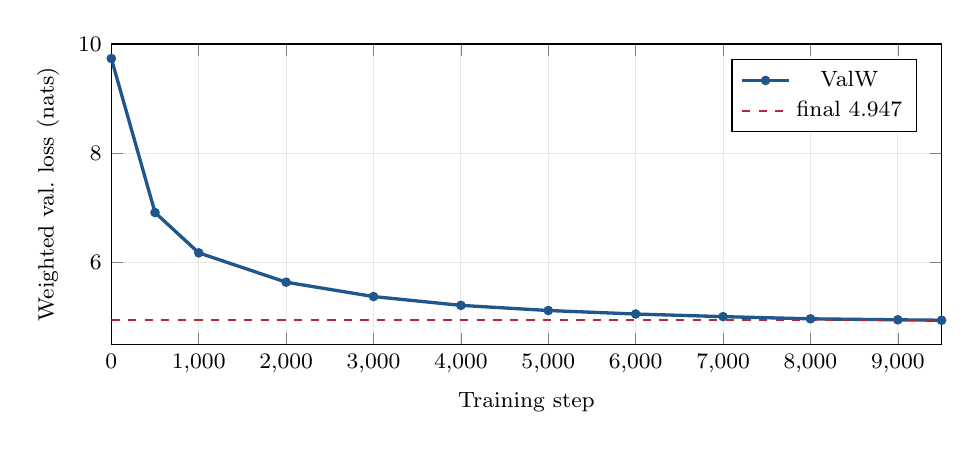
\begin{tikzpicture}
\begin{axis}[
  width=\columnwidth, height=5.4cm,
  xlabel={Training step}, ylabel={Weighted val.\ loss (nats)},
  xmin=0, xmax=9500, ymin=4.5, ymax=10,
  grid=both, grid style={gray!18},
  tick label style={font=\footnotesize},
  label style={font=\footnotesize},
  legend style={font=\footnotesize, at={(0.97,0.95)}, anchor=north east},
]
\addplot[mfblue, very thick, mark=*, mark size=1.1pt] coordinates {
  (0,9.735)(500,6.917)(1000,6.180)(2000,5.643)(3000,5.380)
  (4000,5.219)(5000,5.125)(6000,5.061)(7000,5.013)(8000,4.973)
  (9000,4.955)(9500,4.947)};
\addlegendentry{ValW}
\addplot[mfred, dashed, thick] coordinates {(0,4.947)(9500,4.947)};
\addlegendentry{final 4.947}
\end{axis}
\end{tikzpicture}
\caption{Category-weighted validation loss vs.\ step. The descent is monotone
but flattening, consistent with an approaching capacity/data ceiling rather than
a clean optimisation plateau.}
\label{fig:loss}
\end{figure}

\subsection{Per-category validation loss}
Figure~\ref{fig:cat} shows final per-category perplexity. Grammar/morphology is
the strongest domain (ppl~106) --- it is the most up-weighted (45\% of mix) and
the most formulaic register. Poetry is by far the weakest (ppl~304, $\sim$3$\times$
grammar): partly under-weighting, but structurally the diacritic-stripping
normalisation destroys the vocalisation, meter, and rhyme that poetry depends on.

\begin{figure}[t]
\centering
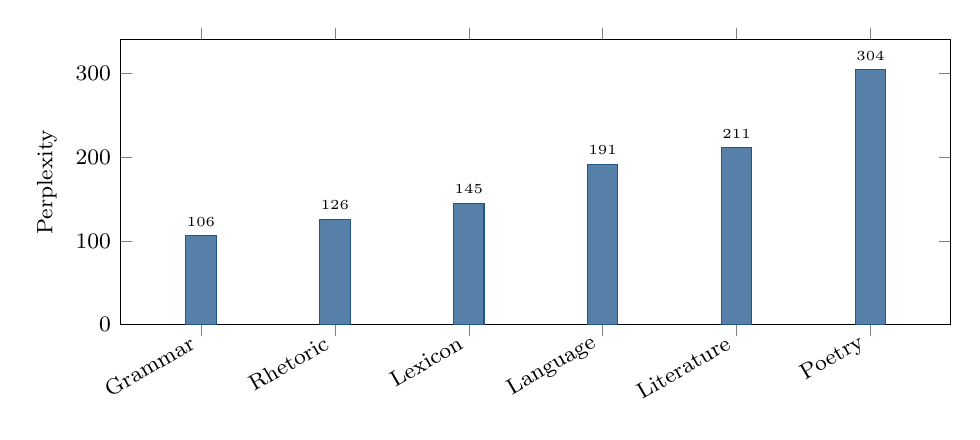
\begin{tikzpicture}
\begin{axis}[
  width=\columnwidth, height=5.2cm,
  ybar, bar width=11pt,
  ylabel={Perplexity}, ymin=0, ymax=340,
  symbolic x coords={Grammar,Rhetoric,Lexicon,Language,Literature,Poetry},
  xtick=data, x tick label style={rotate=30,anchor=east,font=\footnotesize},
  tick label style={font=\footnotesize}, label style={font=\footnotesize},
  nodes near coords, nodes near coords style={font=\tiny},
  enlarge x limits=0.12,
]
\addplot[fill=mfblue!75, draw=mfblue] coordinates {
 (Grammar,106)(Rhetoric,126)(Lexicon,145)(Language,191)(Literature,211)(Poetry,304)};
\end{axis}
\end{tikzpicture}
\caption{Final per-category validation perplexity. Grammar/morphology is
mastered; poetry is the structural outlier, capped by diacritic stripping rather
than by scale alone.}
\label{fig:cat}
\end{figure}

\subsection{Qualitative diagnosis}
The grammar prompt produces locally-correct Arabic but degenerates into
enumerated looping --- the canonical failure mode of an under-capacity model. It
has learned strong local morphological statistics (clean tokens, valid words) but
lacks the representational depth to maintain long-range discourse, so it falls
into high-probability attractor loops. Repetition penalty and nucleus sampling
mask but do not cure this; the fix is capacity~+~data.

\subsection{Hardware efficiency}
Reported MFU is $\approx$0.3\% throughout. At 14.6M parameters and
$\text{block}{=}512$ each step is so cheap that the run is kernel-launch /
Python-overhead bound, not compute-bound. At $\sim$134k~tok/s wall-clock is under
an hour --- but the same GPU could train a 3--5$\times$ larger model, or a far
larger batch, at almost no extra wall-clock cost. This is the strongest argument
that v2 is essentially \emph{free} on the throughput axis.

% ---------------------------------------------------------------- scaling
\section{Why v1 is quality-limited: a scaling-law reading}

\subsection{Chinchilla accounting}
Compute-optimal training scales data with parameters at roughly 20
tokens/parameter~\cite{kaplan,chinchilla}. For v1 the Chinchilla-optimal token
count is $20\times14.6\text{M}=292$M; the model was trained on 655M tokens
(3.8 epochs over 170.7M unique), i.e.\ \emph{past} compute-optimal --- the
correct call for an inference-deployed small model. The binding constraint is
therefore not training length but that 14.6M parameters cannot drive loss below
$\sim$4.9 on this distribution, and that only 170M \emph{unique} tokens exist to
feed a larger model. Both must move together.

\subsection{Locating the data ceiling empirically}
\label{sec:ceiling}
Chinchilla accounting predicts the \emph{compute-optimal} point but not the
\emph{data ceiling} of a \emph{fixed} corpus. To find the latter we run a controlled
scaling sweep --- same 170.7M-token corpus, same tokenizer, same recipe, only model
size varying --- across four weight-tied configurations ($\approx$5M, 15M, 30M, 47M;
$\text{head\_dim}{=}64$ throughout), each trained $\approx$4 epochs with identical
LR-schedule shape and eval cadence. Tying is applied at runtime so v1 reproducibility
is untouched. For each size we record final ValW, the train/val gap, and the
full val-loss curve. The harness (logging, masked per-category eval, checkpointing)
was validated on the 5M pilot before launching the full sweep; the full sweep is run on
an RTX~3090 (bf16). The diagnostic: if ValW keeps falling through 47M, the 170M-token
corpus is \emph{not yet} the binding constraint at that size; if the curve flattens ---
or the train/val gap widens while train loss drops --- the corpus wall has been hit, and
the crossover size is the honest ``best-on-this-data'' point that bounds how far v1's
corpus can be pushed before \emph{more data} (not more parameters) becomes mandatory.

% NOTE TO AUTHOR: scaling_curve.png + numbers are produced by scaling_sweep.py on the
% 3090. The \IfFileExists guard below renders the figure once the run completes; fill
% the empirical crossover sentence after that run. (Harness validated; sweep pending.)
\IfFileExists{scaling_curve.png}{%
\begin{figure}[t]
\centering
\includegraphics[width=\linewidth]{scaling_curve.png}
\caption{Scaling sweep on the fixed 170.7M-token corpus: best weighted validation
loss vs.\ parameter count (weight-tied, $\approx$4 epochs each).}
\label{fig:ceiling}
\end{figure}}{}

\subsection{The weight-tying opportunity}
\label{sec:tying}
Because embeddings dominate the v1 budget, tying the LM head to the input
embedding~\cite{presswolf} is the single highest-leverage change available. It
frees 4.10M parameters (28\% of the model) with negligible quality cost at small
scale, redeploys them into actual computation, and tends to regularise small-vocab
models. The reframed v2 question: do not spend the parameter increase on a third
copy of the vocabulary --- spend it on transformer blocks.

% ---------------------------------------------------------------- comparison
\section{Comparative positioning}
\label{sec:compare}
Table~\ref{tab:compare} situates MiniFrontier among comparable from-scratch and
small decoder-only models.

\begin{table*}[t]
\centering
\small
\caption{Comparative positioning. \textbf{Perplexities across rows are
\emph{not} directly comparable}: they are computed over different tokenizers,
vocabularies, and validation corpora. The table positions MiniFrontier by
parameters, training data, tokenizer, and domain --- not as a leaderboard.
Figures for external models are as reported by their authors.}
\label{tab:compare}
\begin{tabular}{@{}llrrll@{}}
\toprule
Model & Lang. & Params & Train data & Tokenizer / vocab & Reported val.\ ppl \\
\midrule
\textbf{MiniFrontier v1 (ours)} & Arabic (cls.) & \textbf{14.6M} & 170.7M tok ($\times$3.8 ep) & BPE 16k & 141 (weighted) \\
\textbf{MiniFrontier v2 (proposed)} & Arabic (cls.) & \textbf{46.7M} & $\sim$1B tok & BPE 16k & 33--55 (projected) \\
\midrule
Super Tiny LM~\cite{stlm}      & English   & 50M   & --- & BPE & competitive (see paper) \\
SozKZ-50M~\cite{sozkz}         & Kazakh    & 50M   & 9B tok & BPE 50k & benchmark-eval'd \\
GPT-2 small~\cite{gpt2}        & English   & 124M  & WebText & BPE 50k & --- \\
AraGPT2-base~\cite{aragpt2}    & Arabic (MSA) & 135M & 77GB ($\sim$8.8B w) & BPE & under-fits Wiki val.\ \\
113M ``Conventional''~\cite{shapeconv} & English & 113M & Dolma & GPT-NeoX & 38.3 (WikiText) \\
Qwen2-1.5B (Ar.\ FT)~\cite{resourceaware} & Arabic & 1.5B & FT & --- & 4.72 (MSA, char-norm) \\
\bottomrule
\end{tabular}
\end{table*}

Two methodological cousins are most informative. \textbf{SozKZ}~\cite{sozkz}
trains a 50M-and-up Llama-architecture family from scratch for Kazakh with a
dedicated tokenizer and reports consistent gains from 50M to 600M, directly
supporting our scale-up thesis. The \textbf{Super~Tiny LM}~\cite{stlm} programme
targets exactly the 10/50/100M band on consumer GPUs, validating both our scale
and our $<$48h-on-one-GPU constraint. Among Arabic models,
\textbf{AraGPT2-base}~\cite{aragpt2} (135M, MSA, 77GB) is the nearest
architectural relative but is an order of magnitude larger in both parameters and
data, and its authors note it still under-fits its Wikipedia validation set ---
underscoring that even 135M is data-hungry. The 113M decoder
of~\cite{shapeconv} (WikiText ppl 38.3) is a useful English yardstick for the
loss band a well-fed $\sim$100M model reaches, and motivates our v2 target of
ppl~33--55.

\subsection{Measured bits-per-byte}
\label{sec:bpb}
Perplexity is tokenizer-dependent and therefore unfit for cross-model comparison
(hence the caveat on Table~\ref{tab:compare}). Bits-per-byte (BPB) ---
$\text{BPB}=(\text{nats/token}/\ln 2)/(\text{bytes/token})$ --- is tokenizer-invariant.
We \emph{measure} it rather than estimate it: bytes/token is the mean UTF-8 byte length
of each decoded validation token (not an assumed constant), and nats/token is the
mask-aware flat validation cross-entropy (Qur'\=an spans excluded, as in training).
Over the full validation set v1 reaches \textbf{1.25 bits/byte}
(5.07~nats/token~$\div$~5.86~bytes/token; median 6 bytes/token, p10/p90 = 2/10).
The wide p10/p90 spread --- each Arabic character is 2 UTF-8 bytes, so token lengths
range from single-letter clitics to full words --- gives a nominal 0.73--3.66 envelope;
the 1.25 point value (mean bytes/token) is the meaningful figure. Per category, BPB
tracks the loss ordering but is modulated by byte efficiency:

\begin{table}[h]
\centering\small
\caption{Measured BPB by category (validation set). Lower = more compressible.}
\label{tab:bpb}
\begin{tabular}{@{}lrrr@{}}
\toprule
Category & nats/tok & bytes/tok & BPB \\
\midrule
Bal\=agha (rhetoric)        & 4.84 & 6.44 & \textbf{1.09} \\
Na\d{h}w/\d{s}arf (grammar) & 4.68 & 6.00 & 1.12 \\
Ma\^{a}\=ajim (lexicons)    & 4.98 & 5.92 & 1.21 \\
Lugha (language)            & 5.27 & 6.15 & 1.24 \\
Adab (literature)           & 5.33 & 5.64 & 1.36 \\
Shi\^{a}r (poetry)          & 5.70 & 5.05 & \textbf{1.63} \\
\bottomrule
\end{tabular}
\end{table}

\noindent Poetry is both the highest-loss and the least byte-efficient domain (short,
diacritic-bearing tokens stripped to bare consonants), confirming that tashk\=il removal
caps quality precisely where vocalisation carries the signal. These are measured
anchors, not estimates; v2's BPB should be reported the same way for an honest
cross-version comparison.

% ---------------------------------------------------------------- v2
\section{Proposed v2: a 47M-parameter Arabic model}

\subsection{Candidate configurations}
Table~\ref{tab:v2} lists candidates (all $\text{vocab}{=}16000$,
$d_{\text{ff}}{=}\tfrac{8}{3}d$ rounded to a multiple of 64).

\begin{table}[t]
\centering
\small
\caption{v2 candidate configurations. ``Non-emb'' = parameters performing
computation. $\star$ = recommended.}
\label{tab:v2}
\begin{tabular}{@{}clrrrr@{}}
\toprule
Cfg & $d{\times}L$ & Tied & Total & Non-emb & 20$N$ data \\
\midrule
A & $512{\times}10$ & no  & 48.5M & 32.1M & 970M \\
B & $512{\times}12$ & no  & 54.9M & 38.5M & 1.10B \\
$\star$C & $512{\times}12$ & \textbf{yes} & \textbf{46.7M} & \textbf{38.5M} & 935M \\
D & $640{\times}12$ & yes & 69.7M & 59.5M & 1.39B \\
E & $512{\times}14$ & yes & 53.1M & 45.0M & 1.06B \\
\bottomrule
\end{tabular}
\end{table}

\textbf{Recommendation: Config~C} ($n_{\text{embd}}{=}512$,
$n_{\text{layer}}{=}12$, $n_{\text{head}}{=}8$, hidden~1408, weight-tied). At
46.7M total it hits the ``50M'' target yet, thanks to tying, places 38.5M
parameters into computation --- 6$\times$ the 6.4M of v1 --- while keeping the
embedding share at a healthy 17.5\%. Its Chinchilla-optimal data ($\approx$935M
tokens) is a realistic corpus target. Figure~\ref{fig:budget} contrasts the
v1 and v2-C parameter allocation.

\begin{figure}[t]
\centering
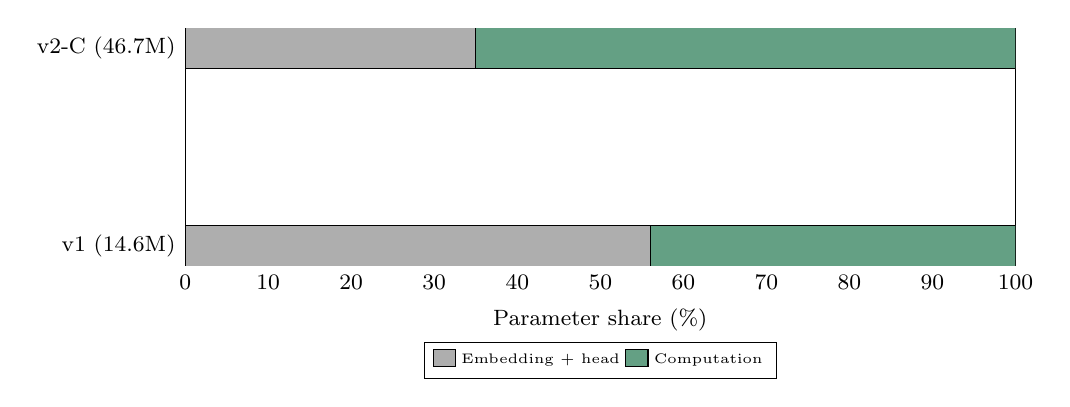
\begin{tikzpicture}
\begin{axis}[
  width=\columnwidth, height=4.6cm,
  xbar stacked, xmin=0, xmax=100,
  ytick={0,1}, yticklabels={v1 (14.6M), v2-C (46.7M)},
  xlabel={Parameter share (\%)},
  tick label style={font=\footnotesize}, label style={font=\footnotesize},
  legend style={font=\tiny, at={(0.5,-0.32)}, anchor=north, legend columns=2},
  bar width=15pt,
]
\addplot[fill=mfgray!60] coordinates {(56.1,0)(35.0,1)};   % embedding share
\addplot[fill=mfgreen!70] coordinates {(43.9,0)(65.0,1)};  % computation share
\legend{Embedding + head, Computation}
\end{axis}
\end{tikzpicture}
\caption{Parameter allocation. Weight tying in v2-C drops the embedding share
from 56\% to $\sim$35\%, redirecting the majority of capacity into computation.}
\label{fig:budget}
\end{figure}

\subsection{Architecture and recipe changes}
The priority changes for v2 are: (1) \textbf{enable weight tying} --- highest ROI
single change; (2) $n_{\text{embd}}\,256{\rightarrow}512$ and
$n_{\text{layer}}\,8{\rightarrow}12$, giving $\text{head\_dim}{=}64$ (the
Flash-Attention sweet spot); (3) optional \textbf{GQA}~\cite{gqa} (e.g.\ 8 query
/ 2 KV heads) to shrink the inference KV-cache; (4) keep RoPE, RMSNorm, SwiGLU,
pre-norm, residual-scale init unchanged; (5) consider
$\text{block\_size}\,512{\rightarrow}1024$ to directly attack looping by
extending discourse history. On the training side: grow the unique corpus to
$\geq$0.9--1.0B tokens (the \#1 lever), raise the micro-batch to 48--96 (MFU
headroom), restore peak LR to $3\!\times\!10^{-4}$ with the larger, calmer batch,
prefer bf16 on the RTX~3090, and de-duplicate aggressively (MinHash/exact) before
counting tokens.

\subsection{Corpus expansion --- the gating dependency}
v2 is bottlenecked by \emph{unique data}, not GPU. Routes to $\sim$1B tokens of
clean Fu\d{s}\d{h}\=a include the Hindawi collection, the Arabic Wikipedia dump,
synthetic textbook-style data in the spirit of ``Textbooks Are All You
Need''~\cite{textbooks}, broadened Shamela categories, and targeted synthetic
generation via the existing local Qwen3 lab for under-represented registers.

\subsection{The diacritics question}
\label{sec:diacritics}
The project's goal is \emph{correct} Arabic, but v1's aggressive
\emph{tashk\=il} stripping caps quality on exactly the dimensions that signal
correctness: case endings (\emph{i\d{q}r\=ab}), voice disambiguation, and all of
poetry. Two paths for v2: (low-risk) keep stripping for bulk pre-training but add
a vocalised sub-corpus (vocalised poetry, the Tashkeela corpus) so the model at
least sees diacritics as in-vocabulary tokens; or (higher-ceiling) train a
diacritisation-aware variant with \emph{tashk\=il} as first-class tokens
throughout --- roughly doubling sequence length, suitable as a v2.x experiment.

% ---------------------------------------------------------------- outcome
\section{Projected outcome and success criteria}
Under Config~C plus a $\sim$1B-token corpus and the recipe above, the scaling-law
expectation is a validation loss of $\approx$3.5--4.0 nats (ppl~$\approx$33--55)
--- roughly a 1.0-nat improvement over v1. We stress this band is a projection, not a
settled floor: the practical floor for tashk\=il-stripped \emph{classical} Arabic is
measurement-pending (the fixed-corpus sweep of Sec.~\ref{sec:ceiling} and the measured
BPB of Sec.~\ref{sec:bpb} are the anchors), and may sit higher than the MSA figures
that motivate the 3.5-nat end of the range. We treat v2 as successful when:
(1)~$\text{ValW}\leq4.0$ and per-category poetry loss $<5.0$ (vs 5.72 today);
(2)~no degenerate looping over $\geq$150 generated tokens at temperature~0.7,
rep.\ penalty~1.1; (3)~MFU~$>$5\% (proof the larger model uses the GPU); and
(4)~embedding share below 20\%. A small ablation grid ---
\{tied vs untied\}$\times$\{12 vs 14 layers\}$\times$\{block 512 vs 1024\},
judged on val loss at a fixed 100M-token budget --- will de-risk the architecture
cheaply before the full run.

% ---------------------------------------------------------------- conclusion
\section{Conclusion}
MiniFrontier v1 is a clean, correctly-engineered small LLaMA: the 2017 attention
core is intact, every surrounding component is a justified modern upgrade, and
the run is stable and reproducible. Its quality is limited by three measurable
factors --- a parameter budget over half-consumed by an untied vocabulary
projection, a 170M-token corpus, and a GPU at 0.3\% utilisation with vast
headroom. The v2 proposal turns each limitation into a lever: tie the embeddings,
double width and depth to $\sim$47M parameters, grow the corpus to $\sim$1B
tokens, and exploit the idle GPU with a larger batch and the restored
$3\!\times\!10^{-4}$ learning rate. The configuration is internally consistent
under Chinchilla scaling and is projected to deliver the step-change in fluency
the project targets --- with diacritisation identified as the key separate axis
required for genuinely correct vocalised Arabic and competent poetry.

% ---------------------------------------------------------------- appendix
\appendix
\section{Generation sample (grammar prompt)}
Under pdflatex the Arabic below may render as boxes; compile with XeLaTeX and the
polyglossia block (see header) to display it. The v1 output begins correctly ---
\texttt{al-f\=aqil marf\=uq wa-qal\=amatu rafqihi al-\d{d}ammah al-\d{z}\=ahirah}
(``the subject is nominative, its marker the visible \d{d}amma'') --- then
degenerates into an enumerated loop, illustrating the under-capacity failure mode
discussed in the body.

% ---------------------------------------------------------------- refs
\begin{thebibliography}{99}
\small
\bibitem{vaswani2017} A.~Vaswani et al. \emph{Attention Is All You Need.} NeurIPS, 2017.
\bibitem{kaplan} J.~Kaplan et al. \emph{Scaling Laws for Neural Language Models.} arXiv:2001.08361, 2020.
\bibitem{chinchilla} J.~Hoffmann et al. \emph{Training Compute-Optimal LLMs (Chinchilla).} arXiv:2203.15556, 2022.
\bibitem{llama} H.~Touvron et al. \emph{LLaMA: Open and Efficient Foundation Language Models.} arXiv:2302.13971, 2023.
\bibitem{rope} J.~Su et al. \emph{RoFormer: Enhanced Transformer with Rotary Position Embedding.} arXiv:2104.09864, 2021.
\bibitem{rmsnorm} B.~Zhang, R.~Sennrich. \emph{Root Mean Square Layer Normalization.} NeurIPS, 2019.
\bibitem{swiglu} N.~Shazeer. \emph{GLU Variants Improve Transformer.} arXiv:2002.05202, 2020.
\bibitem{flash} T.~Dao et al. \emph{FlashAttention.} NeurIPS, 2022.
\bibitem{xiong2020} R.~Xiong et al. \emph{On Layer Normalization in the Transformer Architecture.} ICML, 2020.
\bibitem{presswolf} O.~Press, L.~Wolf. \emph{Using the Output Embedding to Improve Language Models.} EACL, 2017.
\bibitem{adamw} I.~Loshchilov, F.~Hutter. \emph{Decoupled Weight Decay Regularization.} ICLR, 2019.
\bibitem{gqa} J.~Ainslie et al. \emph{GQA: Training Generalized Multi-Query Transformer Models.} arXiv:2305.13245, 2023.
\bibitem{gpt2} A.~Radford et al. \emph{Language Models are Unsupervised Multitask Learners (GPT-2).} OpenAI, 2019.
\bibitem{textbooks} S.~Gunasekar et al. \emph{Textbooks Are All You Need.} arXiv:2306.11644, 2023.
\bibitem{aragpt2} W.~Antoun, F.~Baly, H.~Hajj. \emph{AraGPT2: Pre-Trained Transformer for Arabic Language Generation.} WANLP, arXiv:2012.15520, 2021.
\bibitem{sozkz} S.~Tukenov. \emph{SozKZ: Training Efficient Small Language Models for Kazakh from Scratch.} arXiv:2603.20854, 2026.
\bibitem{stlm} \emph{Super Tiny Language Models.} arXiv:2405.14159, 2024.
\bibitem{shapeconv} \emph{Revisiting the Shape Convention of Transformer Language Models.} arXiv:2602.06471, 2026.
\bibitem{resourceaware} \emph{Resource-Aware Arabic LLM Creation: Model Adaptation, Integration, and Multi-Domain Testing.} arXiv:2412.17548, 2024.
\end{thebibliography}

\end{document}
